\documentclass[../main.tex]{subfiles}
\graphicspath{{\subfix{../IMAGES/}}}

\begin{document}
\localtableofcontents

\subsection{History of Heat Pumps}
Vapor pressure : liquid with own vapor at equilibrium is at saturation pressure $\Rightarrow f(T) = P_{sat}$. Latent heat is absorbed from surroundings to boil.\\
Heat pump allow to gather heat at low temperature and reject it at higher temperature. Can be used to provide cooling/heating. Composed of compressor (increases the working fluid pressure), condenser (rejects heat to high temperature reservoir), expansion valve (decreases working fluid pressure) and evaporator (absorbs heat from low temperature reservoir).\\
Heat is extracted from ground at low temperature and rejected to a house at higher temperature. \\

\subsection{Thermodynamics}
Thermodynamic state properties : m [kg], p [Pa], V$[m^3]$, T [K], U [J], H [J], S[J].\\
A cycle is a sequence of processes leading the system back to initial state. Processes describes closed lines.\\

In closed system, energy can only be transferred through work and heat. If work/heat is provided to the system : $W,Q>0$.\\
\begin{equation}
    \begin{gathered}
        W = -\int pdV\\
        \Delta E = \Delta KE + \Delta PE + \Delta U \Rightarrow E = m(\frac{\omega^2}{2} + gz+ u)\\
        dE = \partial W + \partial Q\\
        \dot{Q} = \int \dot{q}dA \Rightarrow \begin{cases}
            \dot{q} = -\lambda \frac{dT}{dx} & \text{conduction}\\
            \dot{q} = \sigma\varepsilon T^4\: (\sigma = 5.67\cdot 10^{-8}, \varepsilon\in [0,1]) & \text{radiation}\\
            \dot{q} = \alpha(T_{wall} - T_{fluid}) & \text{convection}\\
        \end{cases}
    \end{gathered}
\end{equation}
Internal energy U is the KE related to molecular motion, chemical bonds, intramolecular forces. A change of total energy is a change of state. \\
Convection correlations : \begin{itemize}
    \item forced convection : $Nu = \frac{\alpha L}{\lambda} = f_{forced}(Re,Pr)$
    \item natural convection : $Nu = \frac{\alpha L}{\lambda} = f_{nat} (Gr,Pr)$
    \item Fluid properties : $Pr = \frac{\nu \rho c_p}{\lambda}$, $Re = \frac{vL}{\nu}$, $Gr = \frac{L^3g \beta \Delta T}{\nu^2}$
\end{itemize}
In a cycle : $\Delta E_c = 0 \Rightarrow W_c = -Q_c = -\oint pdV = Q_{hot}^+ - Q_{cold}^-$.\\
\warning Power cycles operate in clockwise direction. 

Typical thermal efficiencies : steam locomotive 0.12, nuclear PP 0.3-0.34, coal plant 0.35-0.48, GT engine 0.3-0.42, CC 0.62, ICE 0.35, large diesel engine 0.58\\
In open system : $\frac{dE_{cv}}{dt} = \dot{W}_{cv} + \dot{Q}_{cv} + \dot{m}_{in}(h+ \frac{w^2}{2} + gz)_{in} - \dot{m}_{out} (h + \frac{w^2}{2} + gz)_{out}$, $h = u+pv$, $v$ the specific volume.\\

Systems left on their own are subject to natural balancing processes until state of equilibrium is reached. \\
Formulation of 2nd law : there is no change of state whose only result is the transfer of heat from a body at lower temperature to a body at higher temperature. (Clausius)\\
A perfect machine is reversible. A process is called reversible if a system can be returned to its initial state without causing any changes in the environment. \\
\warning The thermal efficiency of an irreversible power cycle is lower than that of a reversible cycle. The efficiency of a reversible machine is independent of the process.\\

Thermal efficiency is defined as : $\eta_{th} = 1-\frac{Q^-_{cold}}{Q^+_{hot}} = 1-\frac{T_{cold}}{T_{hot}} = \eta_c$. \warning For a reversible cycle.\\

\begin{figure}[hbt!]
    \centering
    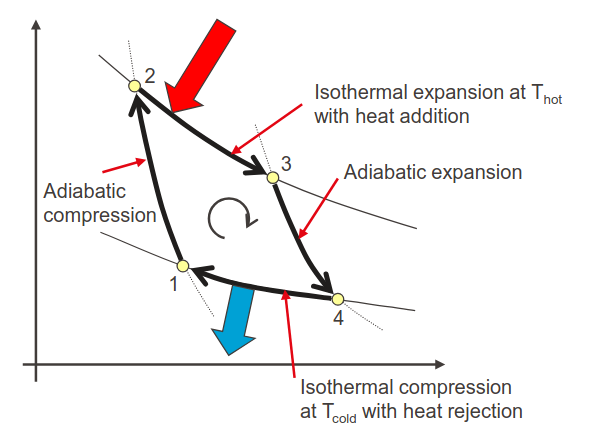
\includegraphics[width=0.5\linewidth]{IMAGES/HP/Screenshot from 2025-02-27 10-55-55.png}
    \caption{Carnot cycle}
\end{figure}
The net work is then : $W_c = (1-\frac{T_c}{T_h}) Q_h$. Maximum thermal efficiency is limited by the Carnot efficiency.\\

\subsubsection{Entropy}
For any cycle process : $\oint \frac{\delta Q}{T} \leq 0$, reversible if : $=0$, irreversible if $<0$, 2nd law forbids processes that $>0$.\\
This can be rewritten as : $\oint \frac{\delta Q}{T} = -\sigma$. The \textbf{entropy} is then a state variable (independent of the process) and $dS = \frac{\delta Q}{T}\rvert_{rev}$.\\
Therefore : $\Delta S = \int \frac{\delta Q}{T} + \sigma$.\\
For an \textbf{open system} : $\frac{dS_{cv}}{dt} = \sum_j \frac{\dot{Q}_j}{T_j} + \sum_{in} \dot{m}s\rvert_{in} - \sum_{out} \dot{m} s\rvert_{out} + \dot{\sigma}_{cv}$.\\
Entropy production(irreversibility) corresponds to lost work.

\subsubsection{Isentropic processes and efficiency}
Often consider adiabatic : $\delta Q = 0, \Delta S=0, \sigma = 0 \Rightarrow$ this is a perfect process.\\
Example (turbine, assume stationary and no change in kinetic/potential energy) : $\dot{m}_{in} = \dot{m}_{out}$, $\dot{W}^-_{cv} = \dot{m}(h_{in}-h_{out})$, $\mathbf{s_{in} - s_{out} = \frac{\dot{\sigma}_{cv}}{\dot{m}}}$. In real process entropy rises due to irreversibility. For isentropic processes : $\dot{W}^-_{cv} = \dot{m}(h_{in} - h_{out,is})$. \warning For compressor, in and out are reversed.\\

The \textbf{isentropic efficiency is then :} (for turbine and compressor) \begin{equation}\begin{gathered}
    \eta_{t-is} = \frac{h_{in}-h_{out}}{h_{in}-h_{out,is}}\\
    \eta_{k-is} = \frac{h_{out,is}-h_{in}}{h_{out}-h_{in}}
    \end{gathered}
\end{equation}

\subsubsection{Exergy}
$1^{st}$ law efficiency leads to an efficiency > 1 for heat pumps. $1^{st}$ law efficiency makes no distinction between quality of energy. Maximum amount of work that you can transform in the system. Exergy is a thermodynamical state variable.\\
Reversible work delivered by the system : $W_{rev} = U_0-U-T_0(S_0-S)- KE-PE$, $W_{use} = W_{rev} + p_0(V_0-V)$.\\

\quad \underline{Closed system :}\\
Exergy in closed system corresponds to useful work : \begin{equation} \begin{gathered}Ex = -W_{use} = (U-U_0) + p_0(V-V_0) - T_0(S-S_0) + KE + PE = (E-E_0)+p_0(V_0-V)-T_0(S-S_0)\\
Ex_2-Ex_1 = E_2-E_1 + p_0(V_2-V_1) - T_0(S_2-S_1) = \int_1^2 (1-\frac{T_0}{T})\delta Q + [W_{12} + p_0(V_2-V_1)] - T_0 \sigma\end{gathered}\end{equation}

\quad \underline{Open system :}\\
Transfer of energy through convection across the boundary. \textbf{Co-enthalpy :} $K = (H-H_0)-T_0(S-S_0)+KE+PE$ (thermodynamic state).\\
\begin{equation} \begin{gathered}k_2-k_1 = (h_2-h_1)-T_0 (s_2-s_1) + \frac{\omega_2^2-\omega_1^2}{2} + g(z_2-z_1)\\
\frac{dEx_{cv}}{dt} = \sum_j \int(1-\frac{T_0}{T_j}) \delta \dot{Q} + \dot{W}_{cv} + p_0 \frac{dV_{cv}}{dt}  + \sum_i \dot{m}_i k_i - \sum_o \dot{m}_o k_o - T_0 \dot{\sigma}_{cv}
\end{gathered}\end{equation}
With $T_0 \dot{\sigma}_{cv} = \dot{L}$ the exergy losses.\\

Example : \begin{itemize}
    \item Fuel boiler : $\dot{Q}_s^+ - \dot{Q}_u^- - \dot{Q}_a^- = 0 \Rightarrow \eta = \frac{\dot{Q}_u^-}{\dot{Q}_s^+}$, $\eta_{ex} = \frac{(1-\frac{T_0}{T_u}) \dot{Q}_u^-}{(1-\frac{T_0}{T_s})\dot{Q}_s^+} = \frac{1-\frac{T_0}{T_u}}{1-\frac{T_0}{T_s}} \eta$
    \item Power cycle : $\dot{Q}_h^+- \dot{Q}_c^- - \dot{W}^- = 0 \Rightarrow \eta = \frac{\dot{W}^-}{\dot{Q}_h^+}$, $\eta_{ex} = \frac{\dot{W}^-}{(1-\frac{T_0}{T_h}) \dot{Q}_h^+} = \frac{\eta_{th}}{\eta_c}$ 
\end{itemize}

\subsection{Power cycles}
Heat pump are bithermal thermodynamic cycle working in anti-clockwise direction. \\
Heating heat pump : heat $q_h$ is delivered at $T_h$. $q_h^- = e^+ + q_a^+$, $\oint dS = 0$, $e^+ = -\oint Pdv + r = -\oint Tds + r$.\\
For a perfect cycle ($r=0$) : $\frac{q_h^-}{T_h} - \frac{q_a^+}{T_a} = 0$, $\frac{q_h^-}{e^+} = \frac{1}{1-\frac{T_a}{T_h}}$. The efficiency (effectiveness) is then : $\frac{q_h^-}{e^+} = \frac{1}{\eta_c} = COP_{carnot\: heat}$. The exergy efficiency is : 
\begin{equation}\begin{gathered}
    \varepsilon = \eta \theta_h\\
    \theta_h = 1-\frac{T_h}{T_c}
    \end{gathered}
\end{equation}

Heating effectiveness increases as $T_h \rightarrow T_a$, goes to  as $T_h \rightarrow \infty$, is $> 1$.\\

Refrigeration heat pump : $q_f^+ = q_a^- - e^+$. \\
Cooling effectiveness is then : $\eta_f = \frac{q_a^-}{e^+} = -\frac{1}{\theta_c} (1-\frac{l}{e^+}) = -\frac{1}{\theta_c} \varepsilon = COP_f$ with $\theta_c = 1-\frac{T_h}{T_c}$. It increases as $T_f \rightarrow T_a$, goes to 0 as $T_f \rightarrow 0$.\\

\quad \underline{How can heat pump cycle be realized? }\\
\begin{itemize}
    \item Reversed stirling cycle (two isothermal and two isochoric processes, internal heat transfer). 
    \begin{figure}[hbt!]
        \centering
        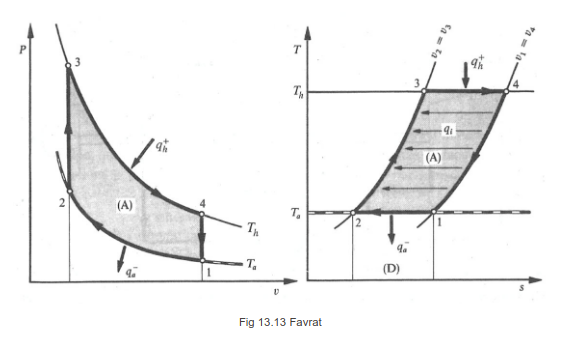
\includegraphics[width=0.5\linewidth]{IMAGES/HP/Screenshot from 2025-03-13 10-19-30.png}
        \caption{Stirling cycle}
    \end{figure}

    \item Reversed ericsson cycle (two isothermal and two isobaric processes, internal heat transfer)
    \begin{figure}[hbt!]
        \centering
        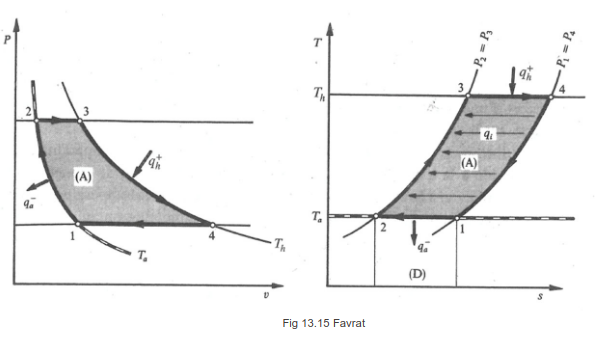
\includegraphics[width=0.5\linewidth]{IMAGES/HP/Screenshot from 2025-03-13 10-21-33.png}
        \caption{Ericsson cycle}
    \end{figure}

    \item Reversed carnot cycle (two isothermal and two isentropic processes, no internal heat transfer). Isothermal compression and expansion are challenging to achieve. Requires isentropic compression and expansion in two phase zone. Liquid in working chamber leads to failure : dry compression is preferred (increase 1 outside of the saturation curve and super heat the fluid above 2). Wet expansion through turbine is difficult and yields low power : use of expansion valve (isenthalpic expansion : 4 is pushed to the right).
\end{itemize}

Components : \begin{itemize}
    \item Compressor : increases pressure from evaporation to condensation, large capacity range
    \item Condenser : rejects heat and condenses working fluid
    \item Expander : reduces pressure from condensation to evaporation level, expander is a throttle valve with variable orifice
    \item Evaporator : absorbs heat and evaporates the working fluid
\end{itemize}

\subsubsection{Analysis of Performance metrics}

\begin{figure}[hbt!]
    \centering
    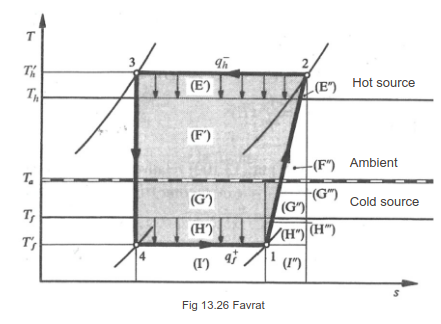
\includegraphics[width=0.5\linewidth]{IMAGES/HP/Screenshot from 2025-03-20 09-32-02.png}
\end{figure}

From energy balance : $q_h^- - q_f^+ = e^+ = r-\oint Tds$. Also, $q_f^+ = T_f'(s_1-s_4) = i'$, $q_h^- = T_h^-(s_2-s_3) = e+f+g+h+i$, $e^+ = (T_h'-T_f')(s_2-s_3)+T_f'(s_2-s_1) = e+f+g+h+i^"$, $-\oint Tds = e'+f'+g'+g^{'''}+h' + h^{'''}$, $r = \int_1^2 Tds = e^"+f^"+g^"+h^"+i^"$.\\
The effectiveness of heating and refrigeration cycle : $\varepsilon_{hf} = \frac{q_h^-+q_f^+}{e^+}$ the definition is disconcerting and meaningless without temperature levels. \\
From exergy balance : $e_{qh}^- + e_{qf}^- = e^+ - (l_{qh} + l_{qf} + l_c + l_e)$, with $e_{qh'}^+ - e_{qh}^- = l_{qh}$, $e_{qh'}^+ = q_h^- (1-\frac{T_a}{T_h^-})$ (received heat exergy), $e_{qh}^- = q_h^- (1-\frac{T_a}{T_h})$ (delivered heat exergy), $l_{qh} = q_h^- (\frac{T_h'-T_h}{T_h'T_h})T_a = \frac{T_a}{T_h}(T_h'-T_h)(s_2-s_3)$. \\
$e_{qf}^+ - e_{qf'}^- = l_{qf}$, $e_{qf'}^+ = q_f^+ (1-\frac{T_a}{T_f})$ (received heat exergy), $e_{qf'}^- = q_f^+ (1-\frac{T_a}{T_f'})$ (delivered heat exergy), $l_{qf} = q_f^+ (\frac{T_f-T_f'}{T_f'T_f})T_a = \frac{T_a}{T_f}(T_f-T_f')(s_1-s_4)$. \\

From the adiabatic compression : $l_c = T_a(s_2-s_1)$.\\
From the expansion : $l_e = T_a(s_4-s_3)$.\\

The exergy efficiency for both heating and cooling is then \begin{equation}\begin{gathered}
    \eta_{ex} = \frac{e_{qh}^-+e_{qf}^+}{e^+} = 1-\frac{T_a}{T_h} [1- \frac{\frac{T_h}{T_f}-1}{\frac{T_h+\Delta T_h}{T_f-\Delta T_f} (1+\frac{\Delta s}{s_1-s_4})-1}]\\
    \Delta T_h = T_h'-T_h\\
    \Delta T_f = T_f-T_f'\\
    \Delta s = s_2-s_1\\
    \end{gathered}
\end{equation}

In case of no dissipation ($\Delta s=0$) and thermal devaluation ($T_f = T_a$) : $\eta_{ex} = \frac{(T_h+\Delta T_h)(T_h-T_a)}{T_h(T_h-T_a+\Delta T_h + \Delta T_f)}$ and the effectiveness : $\varepsilon = \frac{T_h+\Delta T_h}{T_h-T_a + \Delta T_h+ \Delta T_f}$.\\

\subsubsection{Real heat pump}
Single stage vapor compression heat pump : adiabatic compression, condensation with 2K subcooling, isenthalpic expansion valve, evaporation with 2K superheat, cold source is air at $5^\circ C$, hot source is water at $15-90^\circ C$ (10kW), temperature difference on water and air is 5K, pinch in condenser and evaporator is 2K (working fluid ammonia).\\

\begin{figure}[hbt!]
    \centering
    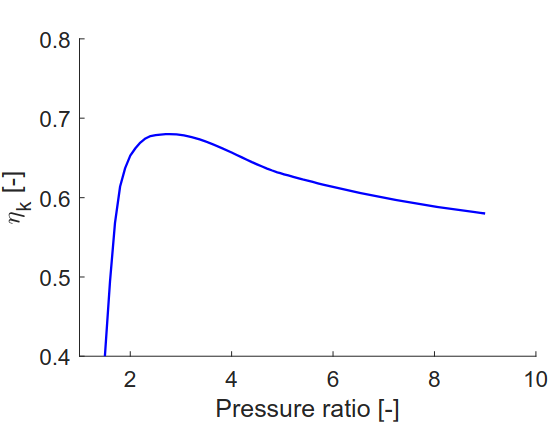
\includegraphics[width=0.5\linewidth]{IMAGES/HP/Screenshot from 2025-03-20 10-25-37.png}
    \caption{Efficiency of the compressor}
\end{figure}
Compressor accounts for $50\%$ of the exergy losses. \\

\begin{figure}[hbt!]
    \centering
    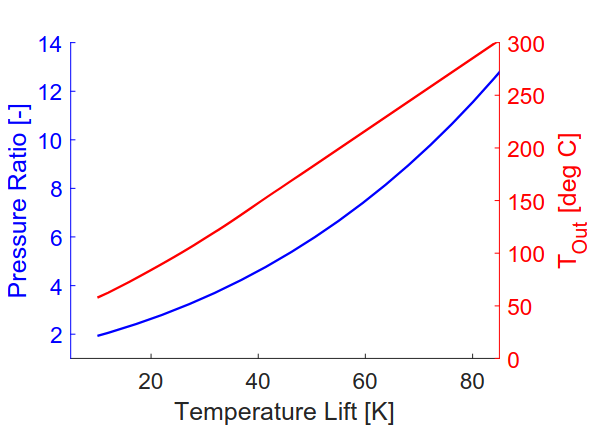
\includegraphics[width=0.5\linewidth]{IMAGES/HP/Screenshot from 2025-03-20 10-35-32.png}
    \caption{Compressor}
\end{figure}
Single stage cycle are well suited for low temperature lifts. Heat exchangers are key for decreasing losses at low lifts. \\

\subsubsection{Improvements}
For the compressor, splitting compression process with intercooling reduces power to achieve same pressure ratio and reduces exhaust temperature. For the expansion : splitting expansion process reduces losses and increases latent heat pickup in evaporator. One could also subcool heat to ambient.\\

Two stage compression heat pump cycle : two compression stages in series, adds 3 components. Efficiency is improved by about $20\%$ at high temperature lifts but makes no sense at low temperature lifts. Condenser losses decrease with twin stage cycle as well as expansion losses. Compressor losses decreases only at high temperature lifts. \\

High exhaust temperatures may damage lubricant, deteriorate working fluid and induce mechanical damage to compressor. They occur when high temperature lifts are required. Compressor must run with vapor. Expansion valve requires liquid fluid (vapor bubbles increase flow resistance). Wide operation range is required for the HP. \\

Use of suction superheater offers operational benefits and safety and may improve cycle efficiency (between evaporator and compressor, internal heat exchange). \\

One can also use intercooling between compressor stages by rejecting heat to ambient (still single stage as only one expander, external intercooling).\\

Partial expansion with intermediate rejection, intercooling between compressor stages by mixing of partially expanded fluid (double stage as two expander and two compressor, different mass flow seen by compressors). \\

Two cycle with open flash tank, cycle benefits from reduced expansion losses, decreased compression work and better compressor efficiency.\\

Two stage cycle with IHEX, to avoid distillation for working fluid mixtures, IHEX with double expansion is applied. \\

Cascade, single stage cycles are superposed and linked with IHEX. Individual working fluids can be used.


\subsection{Working fluids}
Working fluid selection has important effect of cycle design : design pressure ratio, latent heat, slope of sat line, slope of isentropic lines, density, thermophysical properties.\\
Gen 1 (1830-1930) : flammable, toxic/reactive fluids. Solvents and other volatile fluids .\\
Gen 2 (1930-1990) : fluids with no flammability nor toxicity with suitable boiling points. Chlorofluocarbons (CFC, R12), hydrofluorocarbons (HCFC, R22) with less chlorine.\\
Gen 3 (1990-2010) : phase out of CFC to HCFC. Replacement of HCFC to HFC.\\
Gen 4 (2010-) : replacement of HFC to HFO (hydrofluoroolefins). \\

Ideal fluid is a function of reduced evaporation pressure. Performance drops sharply for higher pressures due to saturation dome. \\
State of fluid can be represented by a surface in P,T,v : $F(P,T,v)=0$. Vapor quality is defined as : $x= \frac{m_{vapour}}{m_{vapour} + m_{liquid}}$.\\
\begin{figure}[hbt!]
    \centering
    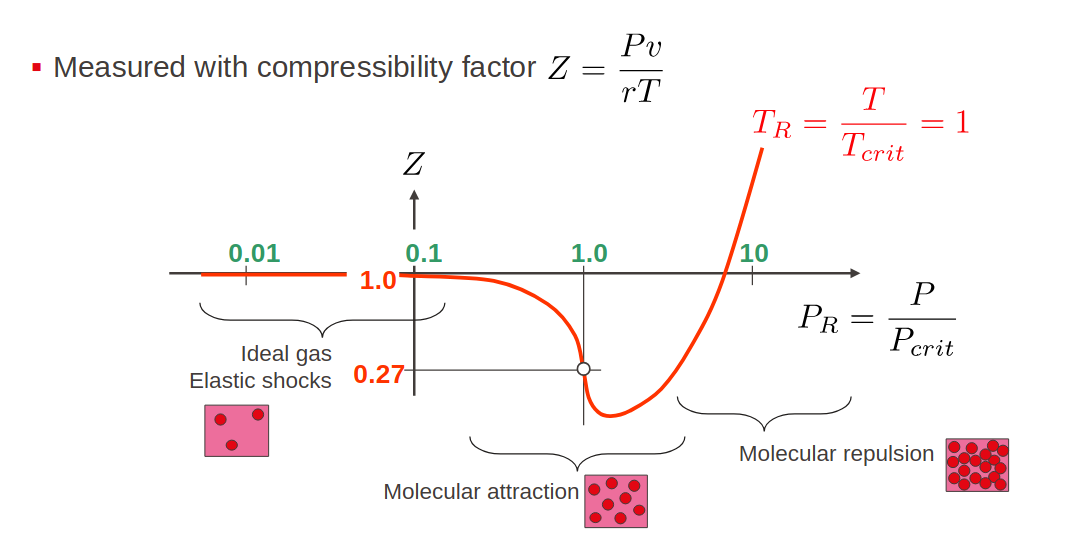
\includegraphics[width=0.5\linewidth]{IMAGES/HP/Screenshot from 2025-04-03 10-04-55.png}
\end{figure}

More accurate equation of state : $P=  \frac{rT}{(v-b)} - \frac{a \alpha}{(v^2 +uvb + wb^2)}$ with Van der Waals ($u=v=0$), Redlich-Kwong ($u=1$, $v=0$), Peng-Robinson ($u=2$, $v=-1$, $\alpha = [1+\kappa (1-T_R^{0.5})]^2$, $\kappa = f_\kappa(w)$, $w = -1-\log_{10} (P_\sigma/P_{crit})$, $P_{\sigma} = P_{sat} @ T_R = 0.7$).\\
Nomenclature : R (M)XYZ(q)\\
number of C : X+1, number of H : Y-1, number of F : Z, M : unsaturated fluid, q : defines molecular arrangement.\\

Multi-component blends : non-azeotropic blends (mixture yields temperature glide during phase change, risk of distillation, poorer heat transfer coefficient), azeotropic blends (mixture yields no temperature glide).\\

\subsection{Compressor technology}

\begin{figure}[hbt!]
    \centering
    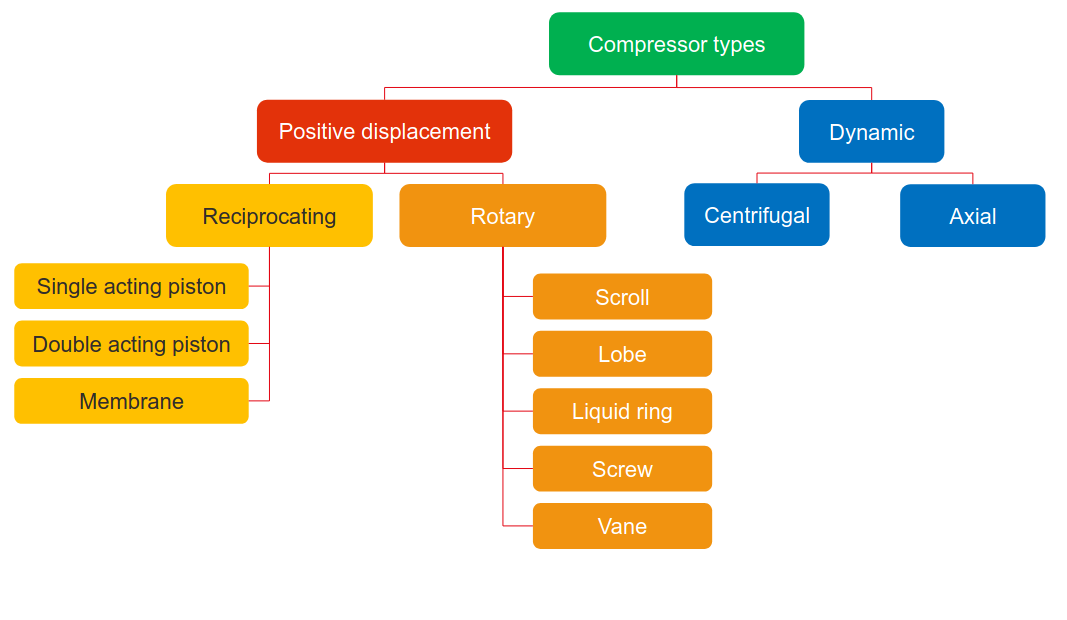
\includegraphics[width=0.5\linewidth]{IMAGES/HP/Screenshot from 2025-04-03 10-35-54.png}
\end{figure}

\begin{figure}[hbt!]
    \centering
    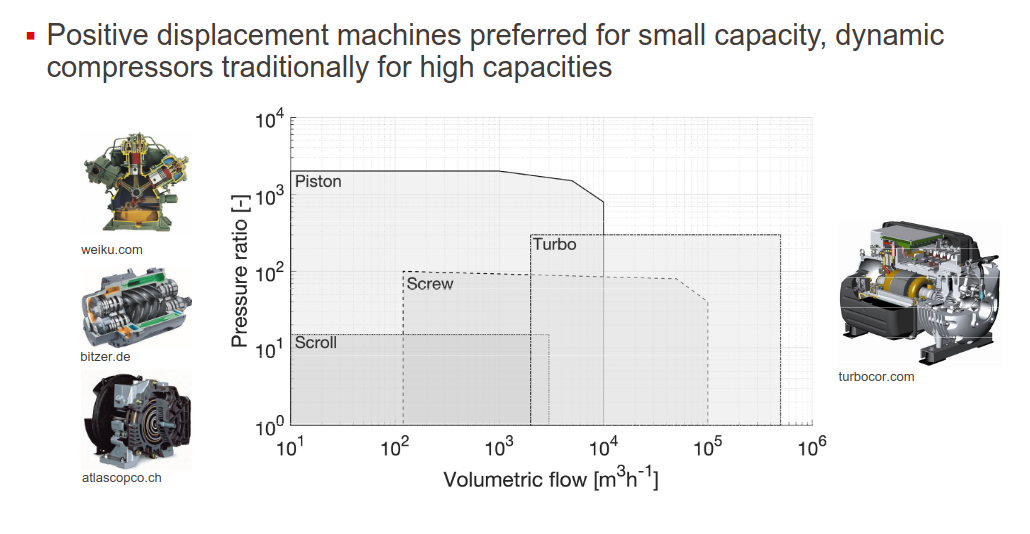
\includegraphics[width=0.5\linewidth]{IMAGES/HP/Screenshot from 2025-04-03 10-39-54.png}
\end{figure}

\subsubsection{Compressor performance}
Ideal compression process : (4-1) isobaric suction ($e^+ = -(v_1-v_4)P_1$), (1-2) compression ($e^+ = -(v_3-v_2)P_2$), (2-3) isobaric discharge ($e^+ = 0$), (3-4) expansion ($e^+ = \frac{1}{1-\kappa} (v_2p_2-v_1p_1)$). 

\begin{figure}[hbt!]
    \centering
    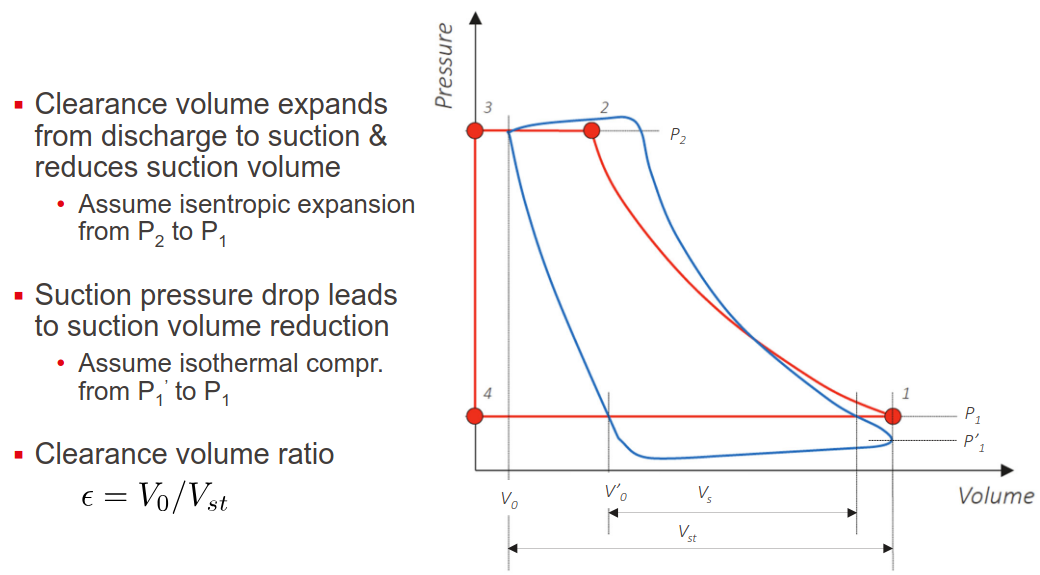
\includegraphics[width=0.5\linewidth]{IMAGES/HP/Screenshot from 2025-04-10 09-38-17.png}
\end{figure}

The total work produced : $e^+ = \frac{\kappa}{\kappa-1} (v_2p_2-v_1p_1) = \frac{\kappa}{\kappa-1} RT_1 [(\frac{P_2}{P_1})^{\frac{\kappa}{\kappa-1}}-1]$.\\

Volumetric efficiency is defined by : $\eta_v = \frac{V_s}{V_{st}} = \eta_{v1} \eta_{v2} \eta_{v3} =\frac{P_1'}{P_1}(1+\varepsilon) - \varepsilon \Pi^{1/\kappa}$, with $\varepsilon = \frac{V_0}{V_{st}}$ and $\Pi = \frac{P_2}{P_1}$, with $\eta_{v1}$ the suction losses, $\eta_{v2}$ the leakage and $\eta_{v3}$ the clearance volume expansion. $\dot{V}_{st} = V_{st} f_c$ with $V_{st}$ the stroke volume and $f_c$ the compressor frequency.\\

The theoretical compressor efficiency for perfect gas : $\eta_{th} = \frac{\kappa[\Pi^{(\kappa-1)/\kappa}-1]}{V_R^{\kappa-1}-\kappa+(\kappa-1)\frac{\Pi}{V_R}}$, with $V_R = \frac{V_{st}}{V_i}$. This takes into account the over/under pressure.\\
$\Pi = V_R^\kappa$.\\

\subsubsection{Screw and scroll compressors}
Heat pumps need to be able to operate under varying conditions. \\
In fixed geometry screw compressors volume ratio and suction volume are defined by geometry of screw rotors and on axial discharge port. By using slide valve the stroke volume of the compressor can be changed. Slide valve at constant width has constant $V_r$ and it is used for power modulation (changes $V_{st}$). Slide valve at varying width modifies $V_r$ while keeping $V_{st}$ constant. 

\subsubsection{Turbocompressors}
A bladed rotating part exchanges work with fluid and stationary bladed part to direct flow. \\
They can be axial (flow parallel to axis of rotation), radial, diagonal, mixed.\\
A stage is the smallest functional entity of turbocompressor. Inducer accelerates fluid into compressor. Rotor transfers energy from shaft to fluid. Multistage pumps are used when required pressure ratio cannot be achieved with one stage.\\

Total torque on the system : $T = \int_{CS} r \times V \rho VdA \Rightarrow T_{shaft} = (r_2V_{t2}-r_1 V_{t1})\dot{m}$ (for homogeneous flow). 
\begin{figure}[hbt!]
    \centering
    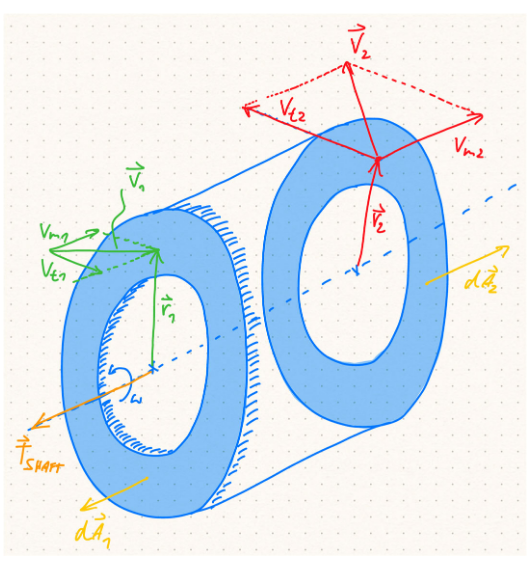
\includegraphics[width=0.5\linewidth]{IMAGES/HP/Screenshot from 2025-04-17 10-21-05.png}
\end{figure}

Euler turbomachinery equation : change of angular momentum about compressor axis between discharge and inlet requires torque $T = \dot{m} (r_4 c_{4u} - r_2 c_{2u})$ (u the tangential component), specific shaft work : $e^+ = w(r_4 c_{4u} - r_2 c_{2u}) = u_4 c_{4u} - u_2 c_{2u}$. It is universally applicable.\\

\begin{figure}[hbt!]
    \centering
    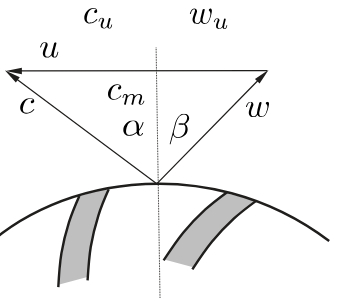
\includegraphics[width=0.5\linewidth]{IMAGES/HP/Screenshot from 2025-04-17 10-36-50.png}
\end{figure}
From the velocity triangle : $c = w+u$, w the rotating velocity, u the tip speed and c the absolute velocity. Then : $e^+ = \frac{1}{2} [(c_4^2-c_2^2) + (w_2^2-w_4^2) + (u_4^2-u_2^2)]$. \\
Turbine : $e^+<0$, compressor : $e^+>0$.\\
Axial machine : $c_{2u} = 0$, $w_4/w_2 = 0.7$, $u_4 \simeq u_2$.\\
Radial machine : $c_{2u} = 0$, $w_4/w_2 = 0.7$, $u_4 \simeq 2 u_2$.\\
In comparison : $w_{2,radial} = w_{2,axial}$, $c_{4u, radial} > c_{4u, axial}$, $u_4 c_{4u,radial} >> u_4 c_{u4,axial}$.\\
\warning Nearly 50\% of the work is due to centrifugal effect (u), radial compressor stage can replace 3-4 axial stages.\\

Assume a radial outflow, no inlet pre-swirl : $\Pi = [Mu^2 (\kappa-1) ]^{\frac{\kappa}{\kappa-1}}$, with $Mu = \frac{u}{a}$ and $a = \sqrt{\kappa R T}$.\\

\subsubsection{Thermodynamics in turbocompressors}
Total enthalpy is given by : $h_0 = h + \frac{c^2}{2}$.\\
Adiabatic work process (turbine, compressor) : $w^+ = \Delta h_0$, diabatic work process : $q^+ + w^+ = \Delta h_0$, adiabatic flow process (constant area pipe flow, diffuser, nozzle) : $\Delta h_0 = 0$, diabatic flow process : $q^+ = \Delta h_0$.\\

Rothalphy is described by : $h + \frac{c^2}{2} - u c_u = I$. It is conserved in a compressor.\\

For a perfect gas : $\frac{P_0}{P} = (\frac{T_0}{T})^{\kappa/(\kappa-1)} = (1+\frac{\kappa-1}{2} M^2)^{\kappa/(\kappa-1)}$. Then : $\frac{\dot{m} \sqrt{RT_0/\kappa}}{AP_0} = M (1+\frac{\kappa-1}{2}M^2)^{-\frac{\kappa+1}{2(\kappa-1)}}$.\\


\subsubsection{Centrifugal compressors}

\begin{figure}[hbt!]
    \centering
    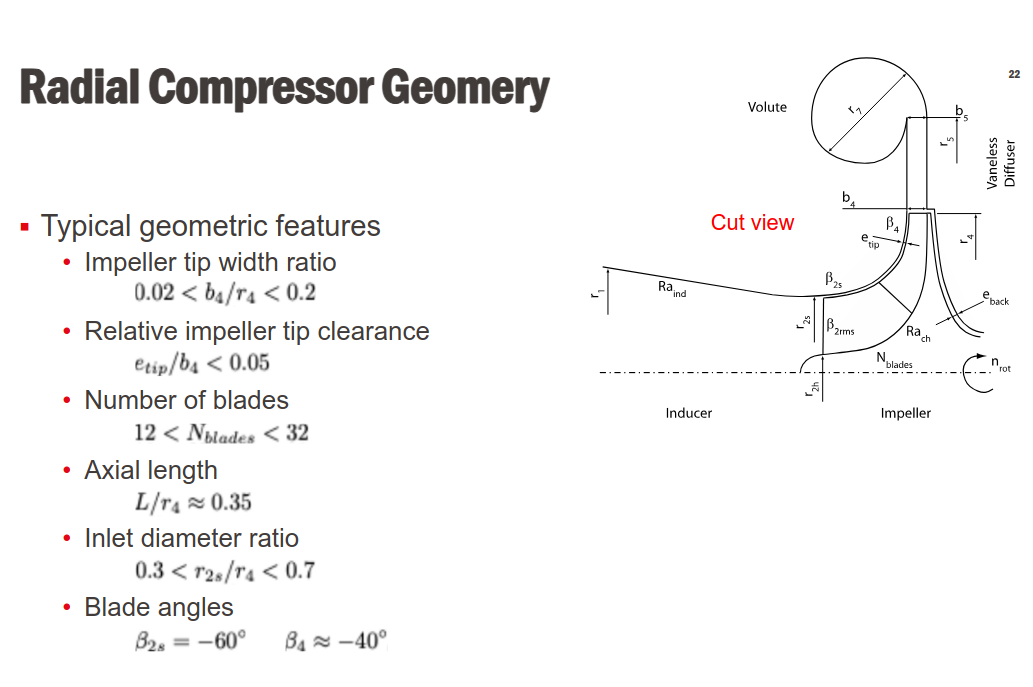
\includegraphics[width=0.5\linewidth]{IMAGES/HP/Screenshot from 2025-05-01 10-31-05.png}
\end{figure}

Chock defines upper mass flow for each speed line. Reducing back pressure increases velocity until it reaches the speed of sound in smallest passage. Further reduction in back pressure yields no increase in mass flow. Speed line is vertical after choking has occurred. Choking can occur at inlet, impeller or diffuser. Higher speed shift choke to higher mass flows until inlet is choked. \\
At surge, mass-flow reduction increases incidence at compressor inlet : flow detaches, inlet recirculation, blockage. Vaneless diffuser stall after inlet recirculation stabilizes, diffuser stall characterized by critical flow angle. Surge line marks the low flow limit of region of stable operation. Instability can have different form : rotating stalls (separation in the blade rows which jumps from one blade to next), mild surge (pulsations in mass flow and pressure without backflow), deep surge (strong periodic backflow through compressor with large pressure and mass flow variations).

\end{document}